\documentclass[twocolumn,superscriptaddress,prb]{revtex4-1}
\usepackage{color}
\usepackage{graphicx}
\usepackage{epstopdf}
\epstopdfsetup{update}
\usepackage{amsmath}
\usepackage{mathtools}
\usepackage[colorlinks,linkcolor=blue,anchorcolor=blue,citecolor=blue,urlcolor=blue]{hyperref}


%===============================================
\begin{document}
\title{Transition from Slater to Mott insulators in Half-Filled SU(6) Hubbard Model on a Square Lattice}
\author{Da Wang} %\email{dawang@nju.edu.cn}
\affiliation{National Laboratory of Solid State Microstructures and School of Physics, Nanjing University, Nanjing 210093, China}
\author{Lei Wang} %\email{wanglei@iphy.ac.cn}
\affiliation{Beijing National Lab for Condensed Matter Physics and Institute of Physics, Chinese Academy of Sciences, Beijing 100190, China}
\author{Congjun Wu} %\email{cjwu@physics.ucsd.edu}
\affiliation{Department of Physics, University of California, San Diego, California 92093, USA}
\begin{abstract}
    Interactions can open single particle gaps by either symmetry breaking or not, called Slater or Mott mechanism, respectively. In this work, we perform large scale projector quantum Monte Carlo simulations to investigate the half-filled SU(6) Hubbard model on the square lattice. By tracing the single particle gap, we find a strong evidence of a crossover from Slater antiferromagnet to Mott antiferromagnetic insulators as $U$ increases. By further increasing $U$, the Mott antiferromagnetic state goes to the Mott valence bond solid state crossing a quantum phase transition which seems to be continuous and thus maybe a deconfined critical point governed by a topological $U(6)/[U(3)\otimes U(3)]$ nonlinear sigma model calling for more elaborated theoretical investigations. 
\end{abstract}
\maketitle

\section{introduction}
For a partially filled electron band, the single particle gap can be opened by either symmetry breaking or interactions, called Slater \cite{Slater_PR_1951} and Mott \cite{Mott_PPSA_1949} insulators, respectively. For the Slater insulator, the single particle gap $\Delta_c$ directly depends on the order parameter. While for the Mott insulator, $\Delta_c$ is roughly proportional to the interaction value and requires no symmetry breaking. However, in a strongly correlated electron system, such two pictures usually blend together. \cite{Imada_RMP_1998,Lee_RMP_2006} For example, in the half-filled Hubbard model on the square lattice, fermi surface nesting leads to Slater antiferromagnetic (AF) state for weak $U$, while the strong $U$ side is effectively described by the Heisenberg model and is attributed to the Mott AF insulator. \cite{Hirsch_PRB_1985} Since there is no more symmetry breaking between the Slater and Mott AF insulators, they are only connected by a crossover. \cite{Pruschke_JPCM_2003} In contrast, in the SU(6) Hubbard model, which is already able to realize in ultracold atom experiments, \cite{Wu_PRL_2003,*Wu_MPLB_2006,Honerkamp_PRL_2004,Assaad_PRB_2005,DeSalvo_PRL_2010,*Taie_PRL_2010,Krauser_NP_2012,*Taie_NP_2012,*Zhang_S_2014,Cazalilla_RPP_2014,*Laflamme_AP_2016} a clear transition from the AF state at weak-$U$ to the valence bond solid (VBS) state at strong-$U$ has been observed via quantum Monte Carlo (QMC) simulations. \cite{Wang_PRL_2014} The weak-$U$ AF is a direct consequence of the fermi surface nesting and Van Hove singularity, while the strong-$U$ VBS is a consequence of the Mott physics. \cite{Zhou_PRB_2016} How such a Slater to Mott transition occurs is an interesting and open question, which is the main aim of the present work.

On the other hand, the quantum phase transition from AF to VBS is predicted to be a continuous one as a result of the deconfined spinons beyond the Landau-Ginzburg-Wilson paradigm. \cite{Senthil_S_2004,*Senthil_PRB_2004,*Levin_PRB_2004} Such a prediction has been supported by some numerical simulations. \cite{Sandvik_PRL_2007,*Melko_PRL_2008,*Sandvik_PRL_2010,*Kaul_PRL_2012,*Pujari_PRL_2013,*Shao_S_2016,*Nahum_PRX_2015,*Wang_PRB_2016,*Assaad_PRX_2016} But there are also other works claiming the first order phase transition and thus violating the prediction. \cite{Kragset_PRL_2006,*Kuklov_AP_2006,*Kuklov_PRL_2008,*Sen_PRB_2010,*Papanikolaou_PRL_2010,*Block_PRL_2013,*DEmidio_PRB_2016,*DEmidio_PRL_2017} As a result, whether the AF to VBS phase transition is a continuous one seems to be model dependent. Another aim of this work is to find out whether the AF to VBS transition in our case is a continuous one, which, if yes, may provide a simple cold atom experimental setup to observe the deconfined critical phenomena. 

Furthermore, another motivation of this work is the AF order here belongs to the self-conjugate representation of the SU(N) spin, which is described by the $U(N)/[U(N/2)\otimes U(N/2)]$ nonlinear sigma model \cite{MacFarlane_PLB_1979,Duerksen_PRD_1981,Read_PRL_1989,*Read_NPB_1989,*Read_PRB_1990}. The symmetry class is different from the widely studied CP$^{N-1}$ model which respects the fundamental representation corresponding to the $U(N)/[U(1)\otimes U(N-1)]$ case. Therefore, the AF phase transition here (if continuous) belongs to a different universality class, the critical exponents of which would be of course desired to characterize such a university class.

\begin{figure} [h]
    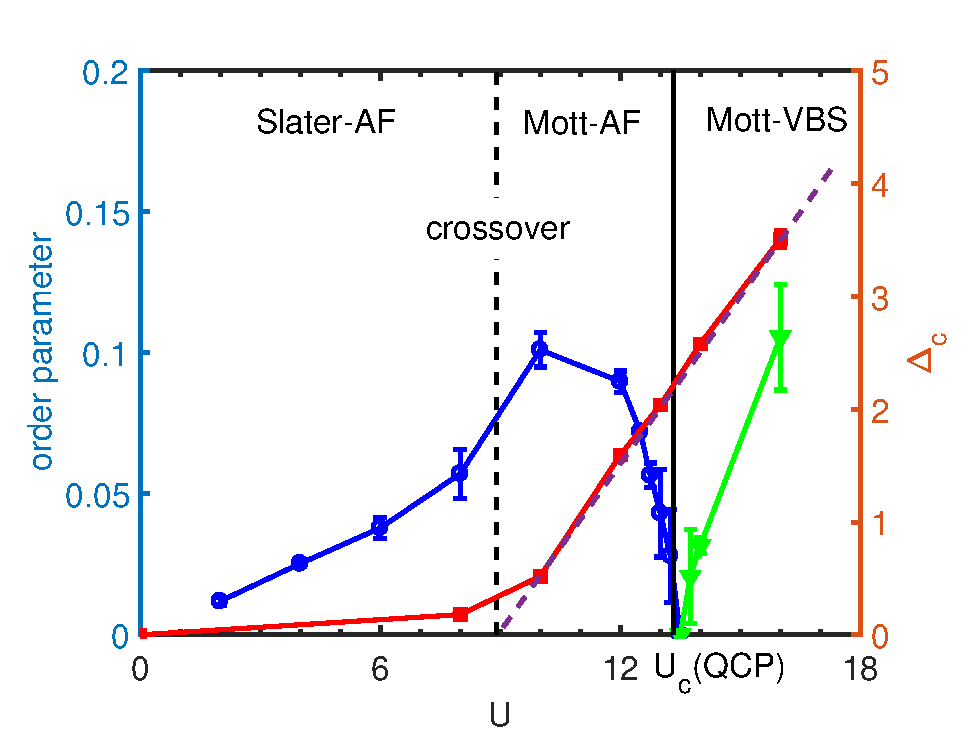
\includegraphics[width=0.5\textwidth]{phasediagram}
    \caption{\label{fig:phasediagram}Phase diagram of the half-filled SU(6) Hubbard model. The AF and VBS order parameters $\langle m \rangle$ and $\langle d \rangle$ are obtained from finite size extrapolations. The values at $U\le8$ are taken from Ref.~\onlinecite{Wang_PRL_2014} directly. The error bars are determined by the $95\%$ confidence bounds of the least square fittings of the finite size data. The single particle gap $\Delta_c$ at $U\ge10$ is extracted from single particle Green's function at $k=(\pi,0)$ and $L=14$, while the data of $U=8$ is taken from Ref.~\onlinecite{Cai_PRB_2013}. The solid black line indicates the transition from AF to VBS which is obtained from the data crossing as shown in Fig.~\ref{fig:correlationlength_af}. The dashed black line is obtained from the linear extrapolation (dashed red line) of $\Delta_c$ at large $U$ and indicates the transition between Slater and Mott insulators.}
\end{figure}

In this work, we apply the projector quantum Monte Carlo free of sign problem to systematically study the half-filled SU(6) Hubbard model on the square lattice. Our main results are shown in Fig.~\ref{fig:phasediagram}. From the slope of single particle gap, we identify a Slater to Mott transition (crossover) around $U^*\approx9$ accompanied by the strong enhancement of the AF order parameter. In the Mott insulator side, the AF to VBS transition occurs at $U_c=13.32(2)$ which seems to be a continuous one as seen from the order parameters and scaling behaviors as in the following discussions. 

%Topological excitations play important roles in modern physics, especially in low dimensions. The deconfinement of vortices in two dimensional XY-model causes the Berezinskii-Kosterlitz-Thouless phase transition. \cite{Kosterlitz1973} While in 2+1 dimensional antiferromagnetic (AF) Heisenberg model, the topological excitations dubbed as hedgehogs can become deconfined and lead the AF phase to a paramagnetic phase by their condensation. \cite{Haldane1988a} Such a magnetic disordering phase can also break lattice symmetry, known as spin-Peierls or valence-bond-solid (VBS) state. \cite{Read1989b,*Read1989a,*Read1990} According to Landau-Ginzburg-Wilson theory, the AF-VBS phase transition should be of first order because they break different symmetries. But from the viewpoint of topological excitations, i.e. hedgehogs in AF and vortices in VBS, the AF-VBS transition is proposed to be a continuous one named as deconfined quantum criticality due to the deconfined topological excitations at the quantum critical point (QCP). \cite{Senthil2004,*Senthil2004a,*Levin2004} The deconfined QCP was first proposed on a non-compact CP$^1$ model and later received much attention in recent years. By many efforts, it has been confirmed numerically on some designer models such as J-Q \cite{Sandvik2007,Melko2008,Sandvik2010,Kaul2012,Pujari2013,Shao2016}, classical loop \cite{Nahum2015}, J$_1$-J$_2$ \cite{Wang2016d} and gauged fermionic \cite{Assaad2016} models. But there are also some other models \cite{Kragset2006,Kuklov2006,Sen2010,Papanikolaou2010} (even including the non compact CP$^1$ model itself\cite{Kuklov2008}) which are found to be of first order and thus may not be deconfined QCPs. 

%The studies have also been extended to higher symmetries, e.g. SO(N)\cite{Kaul2015} and SU(N)
%groups\cite{Lou2009,Kaul2012a,Kaul2012,Block2013,D'Emidio2016,D'Emidio2017}. One motivation is the large-N limit can be solved perturbatively. \cite{Affleck1988a,Marston1989,Arovas1988,Read1989b,*Read1989a,*Read1990,Auerbach2011} Another motivation is that: higher symmetry always brings us more surprises and can unify different phenomena in the sense of low energy effective theories \cite{Hooft2005,Zhang1997,Volovik2003,Hayward2014,Nahum2015a}, or even in bare models directly like in cold atom experiments. \cite{Wu2003,*Wu2006a,DeSalvo2010,Taie2010,Krauser2012,Taie2012,Zhang2014,Cazalilla2014,Laflamme2016} 


%\begin{figure}
%  \begin{flushleft}
%    \includegraphics[width=0.42\textwidth]{su63.jpg}
%    \includegraphics[width=0.30\textwidth]{su61.jpg}
%    \caption{\label{fig:su6}Sketch of SU(6) AF and VBS. (a) and (b) give AF and VBS configurations within the self-conjugate representation which is studied in this work. There are three fermions at each site with flavors represented by six colors.  As a comparison, we also show the fundamental representation in (c) and (d) in which there are one and five fermions at two sublattices, respectively. }
%  \end{flushleft}
%\end{figure}
%


%When talking about SU(N) AF and VBS, we need first to specify their meanings. Mathematically, an SU(N) spin can be
%represented by a Young tableau with $p$ rows and $n_c$ columns of boxes, each of which can be filled with one of N
%values. \cite{Affleck1985,Read1989b,*Read1989a,*Read1990} The extensively studied case in literature
%\cite{Harada2003,Kawashima2007,Lou2009,Kaul2012a,Kaul2012,Block2013,D'Emidio2016,D'Emidio2017} is called fundamental representation with $n_c=p=1$, in which case there is only one particle in A site and $N-1$ particles in B site. The two sites can form a large singlet in the VBS state or keeps frozen to be opposite in the AF state. In large $n_c$ limit, such a representation is a direct generalization of the CP$^{1}$ model, called CP$^{N-1}$ model. \cite{Halperin1974,Read1989b,*Read1989a,*Read1990}
%In this work, we focus on another type of AF and VBS, called self-conjugate representation with $n_c=1$ and $p=N/2$. In this ground state, there are both N/2 particles in A and B sites. 
%%The two sites can form a large singlet by switching one, two and three pairs of particles. 
%To the best of our knowledge, detailed properties of such a AF-VBS transition has received few attentions in literature. \cite{Wang2014b,Lang2015}. By symmetry analysis, from the AF side, the phase transition is known to be described by a $ U(N)/[U(N/2)\otimes U(N/2)]$ nonlinear sigma model \cite{MacFarlane1979,Duerksen1981,Read1989b,*Read1989a,*Read1990} different from the CP$^{N-1}$ model. As a result, it must belong to a new universality class, if the AF-VBS phase transition is really a continuous one. 
%At first sight, let us examine the topological excitations of the self-conjugate VBS state, as plotted in Fig.~\ref{fig:spinon} taking SU(6) case as an example. The vortex is constructed by three fermions (or spinons when charge fluctuations are suppressed), regardless of the VBS types (columnar or plaquette). This is fundamentally different from the CP$^{N-1}$ theory, where the vertex has no internal structure. On the other hand, from the AF side, the phase transition is well known to be described by a non-linear sigma model on a $ U(N)/[U(N/2)\otimes U(N/2)]$ Grassman manifold, \cite{MacFarlane1979,Duerksen1981,Read1989b,*Read1989a,*Read1990} again different from the CP$^{N-1}$ theory. As a result, it is reasonable to expect a new universality class in the self-conjugate representation, if the AF-VBS phase transition is a continuous one. 


%In fact, the self-conjugate represented AF/VBS can readily exist in the half-filled SU(N) Hubbard model, \cite{Honerkamp2004,Assaad2005,Cai2013a,Cai2013,Wang2014b,Zhou2014} \footnote{The SU(N) Hubbard model can also host the fundamental (or generally $p$-rows) represented AF/VBS by choosing different onsite energies on two sublattices to obtain different particle numbers. But this will cause sign problem in determinant QMC and thus prevent large scale calculations.} which has already been realized in cold atom experiments. \cite{Taie2012,Zhang2014,Cazalilla2014} Our previous study\cite{Wang2014b} of this model on a square lattice has identified the existence of AF for small Hubbard $U$ in both SU(4) and SU(6) cases due to Fermi surface nesting and divergence of normal state density of states. However, different from the SU(2) case where the AF moment saturates as $U$ increases, the SU(4) and SU(6) AF moments shows non-monotonic behaviors. For the SU(6) model, AF is eventually killed and substituted by a VBS order. Investigating the critical property of this AF-VBS phase transition is the main task of this work. Through large scale projecting determinant quantum Monte Carlo (QMC) simulations, we have found indications of the deconfined quantum criticality for the self-conjugate represented SU(6) AF-VBS transition. Moreover, the critical exponents indicate the QCP belongs to a new universality class beyond the fundamental represented SU(N) or equivalently non compact CP$^{N-1}$ theory.

%\begin{figure}
%  \includegraphics[width=0.5\textwidth]{spinon}
%  \caption{\label{fig:spinon}Vortex of Z4 VBS. For both columnar and plaquette VBSs, the vortex is a three-fermion state. In low energy theory with charge excitation forbidden, the vortex is constructed by three spinons. Therefore, there are $C_6^3=20$ kinds of vortices altogether.}
%\end{figure}



\section{model and QMC simulations}
The SU(N) Hubbard model on the square lattice is defined as
\begin{eqnarray}
  H=-t\sum_{\langle i,j\rangle,\alpha}\left(c_{i\alpha}^\dag c_{j\alpha}
  +h.c.\right)+\frac{U}{2}\sum_{i}\left(n_i-\frac{N}{2}\right)^2
  \label{eq:hamilton}
\end{eqnarray}
where $c_{i\alpha}$ is a fermion annihilation operator with $i$ the site index and $\alpha$ the flavor index satisfying $1\le\alpha\le N$. The first term represents hoppings between nearest neighbour sites with hopping integral $t$ which is set as $1$ throughout this work. The second term describes the on-site Hubbard interaction and $n_i=\sum_{\alpha=1}^{N} c_{i\alpha}^\dag c_{i\alpha}$. When $N=2$, it goes back to the original Hubbard model. In this work, we focus on the case of $N=6$. 

The half-filling SU(N) (with even N) Hubbard model on a bipartite lattice is free of sign problem in auxiliary field QMC simulations as a result of the particle-hole symmetry, \cite{Wu_PRB_2005,Assaad_PRB_2005} which enables us to perform large scale simulations. Details of the algorithm can be found elsewhere. \cite{Assaad_CMP_2008,Wang_PRL_2014,Zhou_PRB_2016} In our simulations, projection time $\beta=2L$ is used, which is long enough to achieve convergence for a given linear lattice size $L$ up to $24$. The discrete time slice $\Delta\tau$ is chosen to be $0.05$. For each group of parameters, the simulation is performed on 24 cores (48 for $L=24$) with 1000 (500 for $L=24$) Monte Carlo steps to warm up and no less than 1000 (500 for $L=24$) steps for measurement on each core. 



\section{QMC results}

We first present the single particle gap $\Delta_c$ extracted from the slope of $\ln G(\tau,k)$, where $G(\tau,k)$ is the single particle Green's function. The results of $\Delta_c$ at the Van Hove momentum $k=(\pi,0)$ for $L=14$ are shown in Fig.~\ref{fig:phasediagram}. An interesting observation is the nearly linear dependence of $\Delta_c$ on $U$ at $U>U^*\approx 9$, strongly indicating the feature of a Mott insulator. While in the small $U$ side, $\Delta_c$ keeps small values and almost follows the behavior of the AF order parameter which is the main feature of a Slater insulator. 

Next, let us focus on the AF and VBS long range orders. For AF, we define the (diagonal) spin moment operator 
\begin{eqnarray}
  m_r=\frac{1}{6}\left( \sum_{\alpha=1}^{3}n_{r\alpha} -\sum_{\alpha=4}^{6}n_{r\alpha} \right)
\end{eqnarray}
with the largest value $1/2$ the same as SU(2) case. The AF moment is the Fourier component at momentum $(\pi,\pi)$, i.e. $m=\frac{1}{L^2}\sum_{r}m_r(-1)^r$ where the momentum is omitted for simplicity unless otherwise specified. In finite size QMC simulations, symmetry breaking does not happen so we instead measure the equal-time spin-spin correlation directly
\begin{eqnarray}
  \langle m^2 \rangle=\frac{1}{L^4}\sum_{rr'}\langle m_rm_{r'}\rangle (-1)^{r-r'}
\end{eqnarray}

Following Ref.~\onlinecite{Wang_PRL_2014}, to describe the VBS order, we define the kinetic dimer operator
\begin{eqnarray}
  d_{r\hat{e}}=\sum_{\alpha=1}^{6}\left(c_{r\alpha}^\dag c_{r+\hat{e}\alpha} + c_{r+\hat{e}}^\dag c_{r\alpha} \right)
\end{eqnarray}
where $e=x,y$. Then the VBS order parameter is given by $d_e=\frac{1}{L^2}\sum_r d_{r\hat{e}}(-1)^e$. Again, in QMC simulations, we directly measure the dimer-dimer correlation 
\begin{eqnarray}
  \langle d^2 \rangle=\frac{1}{L^4}\sum_{rr'} \langle d_{r\hat{e}}d_{r\hat{e}}\rangle (-1)^{r_e-r_e'}
\end{eqnarray}
In large $U$ limit, the kinetic dimer order is equivalent to the spin-Peierls VBS defined as $d_{r\hat{e}}=\sum_{\alpha\beta}c_{r\alpha}^\dag c_{r\beta} c_{r+\hat{e}\beta}^\dag c_{r+\hat{e}\alpha}$ in SU(N) spin models \cite{Read_PRL_1989,*Read_NPB_1989,*Read_PRB_1990,Marston_PRB_1989} through a second order perturbation process.


\begin{figure}
    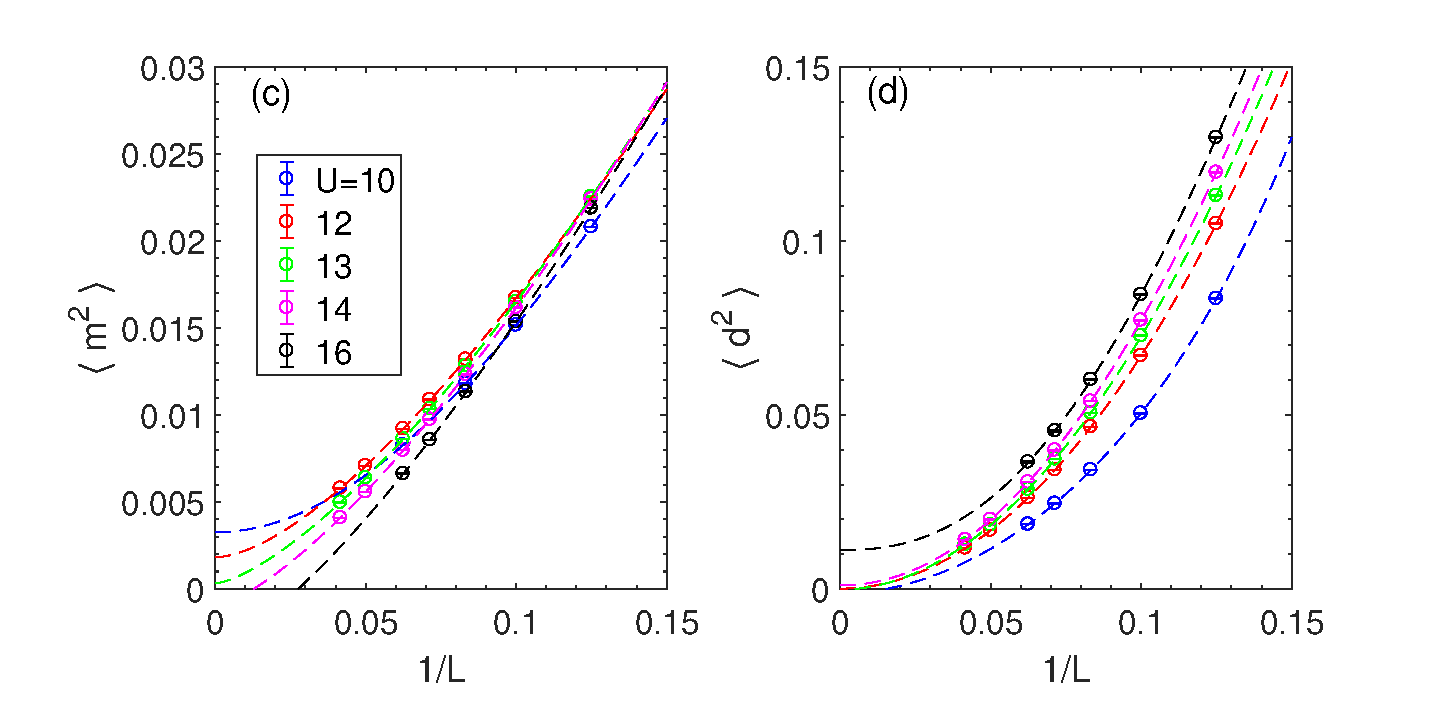
\includegraphics[width=0.5\textwidth]{extrapolation}
    \caption{\label{fig:extrapolation} Finite size extrapolations of $\langle m^2 \rangle$ (a) and $\langle d^2 \rangle$ (b) versus $1/L$ using the power law fitting in Eq.~\ref{eq:fitting}. The logarithmic vertical coordinates are employed to clarify the differences of different interactions.}
\end{figure}

After obtaining $\langle m^2 \rangle$ and $\langle d^2 \rangle$, we perform finite size extrapolation to obtain their thermodynamic limit values. Without the precise knowledge of the finite size effect in prior, we tried different fitting functions. We found the usual polynomial (neither square nor cubic) functions of $1/L$ fail to fit the data. Instead, we found a simple power law function
\begin{eqnarray}\label{eq:fitting}
f(L)=a+\frac{b}{L^c}
\end{eqnarray}
works pretty well, where $a$, $b$, $c$ are fitting parameters. We don't have a good reason for such an unusual but simple extrapolation method. We argue it may because we are working (from $U=10$ to $U=16$) near the quantum phase transition point. The fitting results are shown in Fig.~\ref{fig:extrapolation}. For AF (VBS), as $U$ increases (decreases), the extrapolated value drops from a positive value to negative (no order). Both transitions occur at almost the same $13<U_c<13.5$. The extrapolated order parameters are plotted in Fig.~\ref{fig:phasediagram}. Both AF and VBS order parameters drop near the phase transition and show tendencies to vanish. We have also checked the evolutions of total and kinetic energies (not shown here), neither of which shows a discontinuous behavior. All these results give the signature of a continuous phase transition.


\begin{figure}
	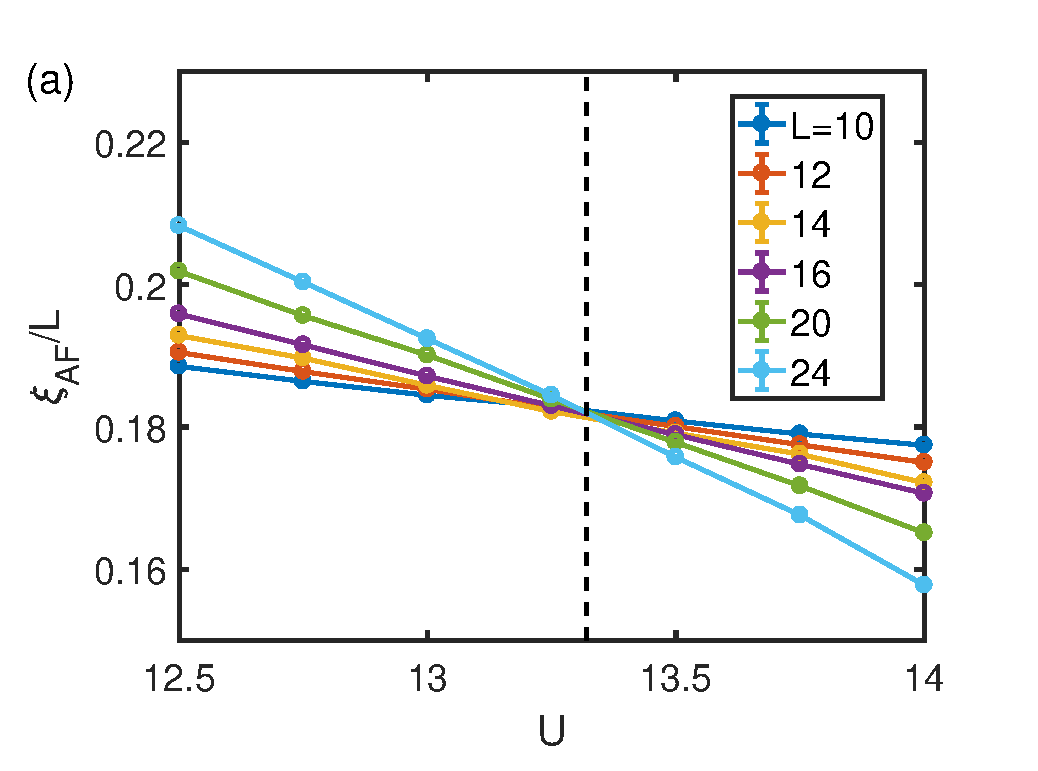
\includegraphics[width=0.4\textwidth]{correlationlength_af}\\
	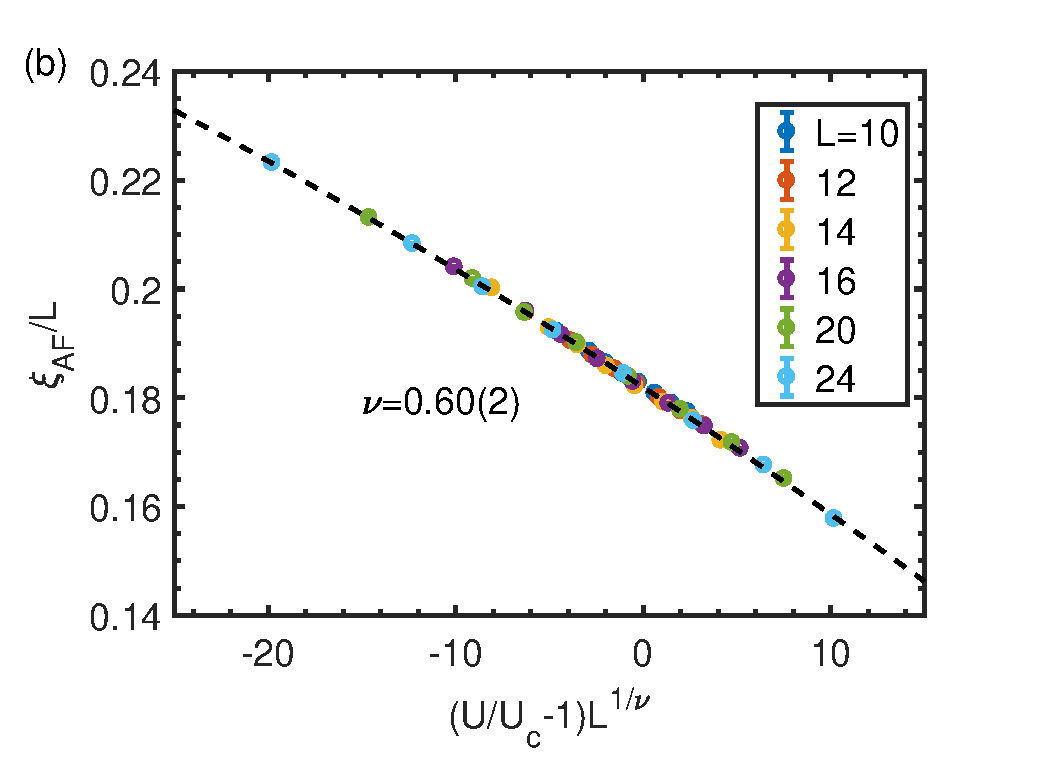
\includegraphics[width=0.4\textwidth]{datacollapse_xi}
	\caption{\label{fig:correlationlength_af} AF correlation length $\xi_{\rm AF}$. (a)$\xi_{\rm AF}/L$ versus $U$ shows a crossing point at $U_c=13.32(2)$. (b)Data collapse of $\xi_{\rm AF}/L$ as a universal function of $(U-U_c)L^{1/\nu}$ with $\nu=0.60(2)$.}
\end{figure}



Next, let us focus on the scaling behavior to check whether the phase transition is indeed a continuous one. From spin-spin correlations, we get the AF correlation length, a good definition of which is \cite{Sandvik_ACP_2010}
\begin{eqnarray}
  \xi_{\rm AF}=\frac{1}{q}\sqrt{\frac{\langle m_Q^2 \rangle}{\langle m_{Q+q}^2 \rangle}-1}
\end{eqnarray}
where $Q=(\pi,\pi)$ and $q=(2\pi/L,0)$. In Fig.~\ref{fig:correlationlength_af}(a), we plot $\xi_{\rm AF}/L$ versus $U$ and find a crossing point at $U_c=13.32(2)$. Furthermore, the $\xi_{\rm AF}$ data are found to collapse to a universal scaling function
\begin{eqnarray}\label{eq:scalinghypothesis}
  \xi_{\rm AF}(U,L)=L f\left[(U-U_c)L^{1/\nu}\right] 
\end{eqnarray}
as plotted in Fig.~\ref{fig:correlationlength_af}(b), where the correlation length exponent $\nu$ is determined to be $0.60(2)$. Such an exquisite scaling behavior strongly indicates the continuous phase transition. 


\begin{figure}
    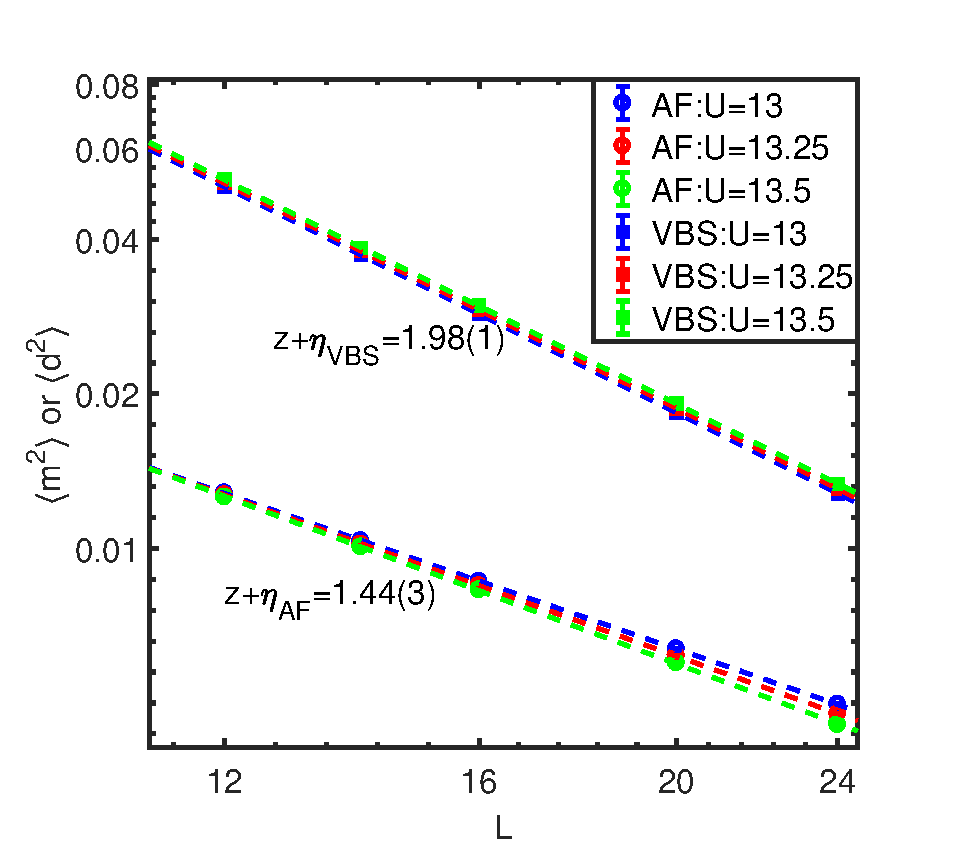
\includegraphics[width=0.45\textwidth]{etaexponent}
    \caption{\label{fig:etaexponent}Anomalous dimensions. We plot $\langle m^2 \rangle$ and $\langle d^2 \rangle$ versus $L$ near the quantum critical point, respectively, using log-log plots. Linear fitting results are shown. }
\end{figure}


At a quantum critical point, two-point correlation function in $2+1$ dimension is expected to be algebraic decay as $\langle m_rm_0\rangle\sim r^{-z-\eta}$ where $z$ and $\eta$ are dynamical exponent and anomalous dimension. \cite{Sondhi_RMP_1997} After Fourier transformation, \begin{eqnarray} \langle m^2 \rangle \sim L^{-z-\eta} \end{eqnarray}
as long as $L$ is large enough. In Fig.~\ref{fig:etaexponent} we plot $\langle m^2 \rangle$ and $\langle d^2\rangle$ versus $L$ on a log-log coordinate around $U_c=13.32(2)$. Up to $L=24$, we find good linear fittings. From the slopes, we obtain $z+\eta_{\rm AF}=1.44(3)$ and $z+\eta_{\rm VBS}=1.98(1)$. In our simulations, the value of $z$ is difficult to determine since it requires the time evolutions of two particle Green's functions which, however, tend to be gapless at the critical point. If we suppose $z=1$ directly following the prediction of deconfined critical theory, \cite{Senthil_S_2004,*Senthil_PRB_2004,*Levin_PRB_2004} we get $\eta_{\rm AF}=0.44(3)$ and $\eta_{\rm VBS}=0.98(1)$ which are different from the SU(6) $J-Q$ model (equivalent to the non-compact CP$^5$ model), \cite{Kaul_PRL_2012} indicating they indeed belong to different universality classes. 




\section{summary and discussion}
In summary, we have performed large scale projector QMC simulations on the half-filled SU(6) Hubbard model. As $U$ increases, we found a crossover at $U^*\approx9$ from Slater-AF to Mott-AF insulators and then a (signature of) continuous phase transition at $U_c=13.32(2)$ from the Mott-AF to Mott-VBS states. 

Several indications or remarks of these numerical observations are given as follows: 
% finite size scaling
(1)The finite size extrapolation in this work is based on the power law fitting in Eq.~\ref{eq:fitting}, which is different from the SU(2) Heisenberg model where the cubic-order polynomial works very well. \cite{Neuberger_PRB_1989,*Sandvik_PRB_1997} Whether the difference comes from the higher symmetry group $SU(N)$ is still an open question, which requires sophisticated knowledge of the excitation properties of the SU(N) Hubbard or Heisenberg model. 
% Mott transition? vs N? vs U?
(2)The threshold $U^*$ for the Mott insulator is argued to be proportional to $N$. \cite{Zhou_PRB_2016}
% Slater-VBS in honeycomb?
(3)In this study, the Mott transition (crossover) is found to reside in the AF phase. However, in the SU(4) honeycomb lattice, AF order is found to disappear and the semimetal phase at weak $U$ goes to VBS directly, where the Mott transition seems to be inside the VBS phase. \cite{Zhou_PRB_2016} Then, there should be a Slater-VBS which is interesting since it cannot be explained by fermi surface nesting or superexchange mechanism in the Mott picture. 
% two-length scaling?
(4)We have also tried to obtain the universal plots of $L^{z+\eta_{\rm AF}}\langle m^2 \rangle$ and $L^{z+\eta_{\rm VBS}}\langle d^2 \rangle$ versus $(U-U_c)L^{1/\nu}$ but failed. Of course, this may be caused by small lattice size in our QMC simulations. But another more physically relevant reason may be the recently proposed two-length scaling hypothesis \cite{Shao_S_2016} while our QMC simulations with small size up to $L=24$ prevent us to perform such an ingenious scaling analysis.
% beyond CP^{N-1}
(5)By symmetry analysis, the observed AF-VBS phase transition belongs to a broader universality class governed by a $U(N)/[U(m)\otimes U(N-m)]$ nonlinear sigma model beyond the CP$^{N-1}$ model corresponding to $m=1$. The full understanding, e.g. critical exponents, of the $m>1$ models calls for more elaborated theoretical efforts, e.g. $1/N$ expansion \cite{Wang_a_2018} or renormalization group analysis in the future.


\section{acknowledgement}
We thank xxx.
We are supported by grant yyy.
Our numerical calculations are performed on Tianhe-II. 

\bibliography{su6dqcp}
\end{document}
